% Options for packages loaded elsewhere
\PassOptionsToPackage{unicode}{hyperref}
\PassOptionsToPackage{hyphens}{url}
%
\documentclass[
]{article}
\usepackage{amsmath,amssymb}
\usepackage{lmodern}
\usepackage{ifxetex,ifluatex}
\ifnum 0\ifxetex 1\fi\ifluatex 1\fi=0 % if pdftex
  \usepackage[T1]{fontenc}
  \usepackage[utf8]{inputenc}
  \usepackage{textcomp} % provide euro and other symbols
\else % if luatex or xetex
  \usepackage{unicode-math}
  \defaultfontfeatures{Scale=MatchLowercase}
  \defaultfontfeatures[\rmfamily]{Ligatures=TeX,Scale=1}
\fi
% Use upquote if available, for straight quotes in verbatim environments
\IfFileExists{upquote.sty}{\usepackage{upquote}}{}
\IfFileExists{microtype.sty}{% use microtype if available
  \usepackage[]{microtype}
  \UseMicrotypeSet[protrusion]{basicmath} % disable protrusion for tt fonts
}{}
\makeatletter
\@ifundefined{KOMAClassName}{% if non-KOMA class
  \IfFileExists{parskip.sty}{%
    \usepackage{parskip}
  }{% else
    \setlength{\parindent}{0pt}
    \setlength{\parskip}{6pt plus 2pt minus 1pt}}
}{% if KOMA class
  \KOMAoptions{parskip=half}}
\makeatother
\usepackage{xcolor}
\IfFileExists{xurl.sty}{\usepackage{xurl}}{} % add URL line breaks if available
\IfFileExists{bookmark.sty}{\usepackage{bookmark}}{\usepackage{hyperref}}
\hypersetup{
  pdftitle={PF\_1\_2},
  hidelinks,
  pdfcreator={LaTeX via pandoc}}
\urlstyle{same} % disable monospaced font for URLs
\usepackage[margin=1in]{geometry}
\usepackage{color}
\usepackage{fancyvrb}
\newcommand{\VerbBar}{|}
\newcommand{\VERB}{\Verb[commandchars=\\\{\}]}
\DefineVerbatimEnvironment{Highlighting}{Verbatim}{commandchars=\\\{\}}
% Add ',fontsize=\small' for more characters per line
\usepackage{framed}
\definecolor{shadecolor}{RGB}{248,248,248}
\newenvironment{Shaded}{\begin{snugshade}}{\end{snugshade}}
\newcommand{\AlertTok}[1]{\textcolor[rgb]{0.94,0.16,0.16}{#1}}
\newcommand{\AnnotationTok}[1]{\textcolor[rgb]{0.56,0.35,0.01}{\textbf{\textit{#1}}}}
\newcommand{\AttributeTok}[1]{\textcolor[rgb]{0.77,0.63,0.00}{#1}}
\newcommand{\BaseNTok}[1]{\textcolor[rgb]{0.00,0.00,0.81}{#1}}
\newcommand{\BuiltInTok}[1]{#1}
\newcommand{\CharTok}[1]{\textcolor[rgb]{0.31,0.60,0.02}{#1}}
\newcommand{\CommentTok}[1]{\textcolor[rgb]{0.56,0.35,0.01}{\textit{#1}}}
\newcommand{\CommentVarTok}[1]{\textcolor[rgb]{0.56,0.35,0.01}{\textbf{\textit{#1}}}}
\newcommand{\ConstantTok}[1]{\textcolor[rgb]{0.00,0.00,0.00}{#1}}
\newcommand{\ControlFlowTok}[1]{\textcolor[rgb]{0.13,0.29,0.53}{\textbf{#1}}}
\newcommand{\DataTypeTok}[1]{\textcolor[rgb]{0.13,0.29,0.53}{#1}}
\newcommand{\DecValTok}[1]{\textcolor[rgb]{0.00,0.00,0.81}{#1}}
\newcommand{\DocumentationTok}[1]{\textcolor[rgb]{0.56,0.35,0.01}{\textbf{\textit{#1}}}}
\newcommand{\ErrorTok}[1]{\textcolor[rgb]{0.64,0.00,0.00}{\textbf{#1}}}
\newcommand{\ExtensionTok}[1]{#1}
\newcommand{\FloatTok}[1]{\textcolor[rgb]{0.00,0.00,0.81}{#1}}
\newcommand{\FunctionTok}[1]{\textcolor[rgb]{0.00,0.00,0.00}{#1}}
\newcommand{\ImportTok}[1]{#1}
\newcommand{\InformationTok}[1]{\textcolor[rgb]{0.56,0.35,0.01}{\textbf{\textit{#1}}}}
\newcommand{\KeywordTok}[1]{\textcolor[rgb]{0.13,0.29,0.53}{\textbf{#1}}}
\newcommand{\NormalTok}[1]{#1}
\newcommand{\OperatorTok}[1]{\textcolor[rgb]{0.81,0.36,0.00}{\textbf{#1}}}
\newcommand{\OtherTok}[1]{\textcolor[rgb]{0.56,0.35,0.01}{#1}}
\newcommand{\PreprocessorTok}[1]{\textcolor[rgb]{0.56,0.35,0.01}{\textit{#1}}}
\newcommand{\RegionMarkerTok}[1]{#1}
\newcommand{\SpecialCharTok}[1]{\textcolor[rgb]{0.00,0.00,0.00}{#1}}
\newcommand{\SpecialStringTok}[1]{\textcolor[rgb]{0.31,0.60,0.02}{#1}}
\newcommand{\StringTok}[1]{\textcolor[rgb]{0.31,0.60,0.02}{#1}}
\newcommand{\VariableTok}[1]{\textcolor[rgb]{0.00,0.00,0.00}{#1}}
\newcommand{\VerbatimStringTok}[1]{\textcolor[rgb]{0.31,0.60,0.02}{#1}}
\newcommand{\WarningTok}[1]{\textcolor[rgb]{0.56,0.35,0.01}{\textbf{\textit{#1}}}}
\usepackage{graphicx}
\makeatletter
\def\maxwidth{\ifdim\Gin@nat@width>\linewidth\linewidth\else\Gin@nat@width\fi}
\def\maxheight{\ifdim\Gin@nat@height>\textheight\textheight\else\Gin@nat@height\fi}
\makeatother
% Scale images if necessary, so that they will not overflow the page
% margins by default, and it is still possible to overwrite the defaults
% using explicit options in \includegraphics[width, height, ...]{}
\setkeys{Gin}{width=\maxwidth,height=\maxheight,keepaspectratio}
% Set default figure placement to htbp
\makeatletter
\def\fps@figure{htbp}
\makeatother
\setlength{\emergencystretch}{3em} % prevent overfull lines
\providecommand{\tightlist}{%
  \setlength{\itemsep}{0pt}\setlength{\parskip}{0pt}}
\setcounter{secnumdepth}{-\maxdimen} % remove section numbering
\ifluatex
  \usepackage{selnolig}  % disable illegal ligatures
\fi

\title{PF\_1\_2}
\author{}
\date{\vspace{-2.5em}}

\begin{document}
\maketitle

\begin{Shaded}
\begin{Highlighting}[]
\FunctionTok{library}\NormalTok{(tidyverse)}
\FunctionTok{library}\NormalTok{(mosaic)}
\FunctionTok{library}\NormalTok{(readxl)}
\FunctionTok{library}\NormalTok{(lmtest)}
\end{Highlighting}
\end{Shaded}

\begin{Shaded}
\begin{Highlighting}[]
\NormalTok{data\_ex2 }\OtherTok{\textless{}{-}} \FunctionTok{read\_excel}\NormalTok{(}\StringTok{"data/freqdata.xlsx"}\NormalTok{)}
\FunctionTok{head}\NormalTok{(data\_ex2)}
\end{Highlighting}
\end{Shaded}

\begin{verbatim}
## # A tibble: 6 x 25
##     obs  year period state   age fatal  male female single multiple lnpop lnpopm
##   <dbl> <dbl>  <dbl> <dbl> <dbl> <dbl> <dbl>  <dbl>  <dbl>    <dbl> <dbl>  <dbl>
## 1     1  1990      1     1    16    16     8      8     11        5  11.0   10.3
## 2     2  1991      2     1    16    20    14      6     16        4  11     10.3
## 3     3  1992      3     1    16    14     9      5      6        8  11.0   10.3
## 4     4  1993      4     1    16    14    10      4      9        5  11.0   10.4
## 5     5  1994      5     1    16    22    14      8     14        8  11.0   10.4
## 6     6  1995      6     1    16    23    14      9     14        9  11.0   10.4
## # ... with 13 more variables: lnpopf <dbl>, unempl <dbl>, gdl <dbl>,
## #   gdl3 <dbl>, gdl2 <dbl>, gdl1 <dbl>, beltsc <dbl>, beltpr <dbl>,
## #   bac08 <dbl>, zerotol <dbl>, alr <dbl>, sp70 <dbl>, sp65 <dbl>
\end{verbatim}

\hypertarget{section-a}{%
\section{--------------------- Section A
-----------------------------}\label{section-a}}

\emph{Make descriptive statistics, e.g.~a table with summary statistics
and a correlation matrix, and discuss the results, for the variables
that you are going to use (read the whole exercise first to decide which
variables are relevant in the descriptive statistics).}

\begin{Shaded}
\begin{Highlighting}[]
\NormalTok{fav\_df }\OtherTok{\textless{}{-}} \FunctionTok{rbind}\NormalTok{(}
  \FunctionTok{favstats}\NormalTok{(data\_ex2}\SpecialCharTok{$}\NormalTok{lnpop),}
  \FunctionTok{favstats}\NormalTok{(data\_ex2}\SpecialCharTok{$}\NormalTok{unempl),}
  \FunctionTok{favstats}\NormalTok{(data\_ex2}\SpecialCharTok{$}\NormalTok{sp65),}
  \FunctionTok{favstats}\NormalTok{(data\_ex2}\SpecialCharTok{$}\NormalTok{gdl),}
  \FunctionTok{favstats}\NormalTok{(data\_ex2}\SpecialCharTok{$}\NormalTok{bac08),}
  \FunctionTok{favstats}\NormalTok{(data\_ex2}\SpecialCharTok{$}\NormalTok{beltsc),}
  \FunctionTok{favstats}\NormalTok{(data\_ex2}\SpecialCharTok{$}\NormalTok{beltpr),}
  \FunctionTok{favstats}\NormalTok{(data\_ex2}\SpecialCharTok{$}\NormalTok{zerotol),}
  \FunctionTok{favstats}\NormalTok{(data\_ex2}\SpecialCharTok{$}\NormalTok{alr)}
\NormalTok{)}
\FunctionTok{row.names}\NormalTok{(fav\_df) }\OtherTok{\textless{}{-}} \FunctionTok{c}\NormalTok{(}\StringTok{"ln(population)"}\NormalTok{, }\StringTok{"unemployment rate"}\NormalTok{, }\StringTok{"speed limit 65"}\NormalTok{, }\StringTok{"graduated driver license law"}\NormalTok{, }\StringTok{"Blood alcohol \textless{} 0.08 law"}\NormalTok{, }\StringTok{"Secondary seat belt law"}\NormalTok{, }\StringTok{"Primary seat belt law"}\NormalTok{, }\StringTok{"Zero tolerance alcohol law"}\NormalTok{, }\StringTok{"License revocation law"}\NormalTok{)}
\NormalTok{fav\_df  }\SpecialCharTok{\%\textgreater{}\%} \FunctionTok{mutate}\NormalTok{(}\FunctionTok{across}\NormalTok{(}\FunctionTok{where}\NormalTok{(is.numeric), }\SpecialCharTok{\textasciitilde{}} \FunctionTok{round}\NormalTok{(., }\DecValTok{4}\NormalTok{)))}
\end{Highlighting}
\end{Shaded}

\begin{verbatim}
##                               min      Q1 median    Q3   max    mean     sd   n
## ln(population)               8.85 10.1875  10.96 11.41 13.23 10.8533 0.9703 960
## unemployment rate            2.30  4.2000   5.10  6.10 13.40  5.2497 1.5815 960
## speed limit 65               0.00  0.0000   1.00  1.00  1.00  0.5490 0.4979 960
## graduated driver license law 0.00  0.0000   0.00  1.00  1.00  0.4500 0.4978 960
## Blood alcohol < 0.08 law     0.00  0.0000   0.00  1.00  1.00  0.4781 0.4998 960
## Secondary seat belt law      0.00  1.0000   1.00  1.00  1.00  0.9052 0.2931 960
## Primary seat belt law        0.00  0.0000   0.00  1.00  1.00  0.2771 0.4478 960
## Zero tolerance alcohol law   0.00  0.0000   1.00  1.00  1.00  0.7104 0.4538 960
## License revocation law       0.00  0.0000   1.00  1.00  1.00  0.5490 0.4979 960
##                              missing
## ln(population)                     0
## unemployment rate                  0
## speed limit 65                     0
## graduated driver license law       0
## Blood alcohol < 0.08 law           0
## Secondary seat belt law            0
## Primary seat belt law              0
## Zero tolerance alcohol law         0
## License revocation law             0
\end{verbatim}

favstats(data\_ex2\(lnpop),  favstats(data_ex2\)unempl),
favstats(data\_ex2\(sp65),  favstats(data_ex2\)gdl),
favstats(data\_ex2\(bac08),  favstats(data_ex2\)beltsc),
favstats(data\_ex2\(beltpr),  favstats(data_ex2\)zerotol),
favstats(data\_ex2\$alr)

\begin{Shaded}
\begin{Highlighting}[]
\NormalTok{data\_ex2 }\SpecialCharTok{\%\textgreater{}\%} \FunctionTok{select}\NormalTok{(}\FunctionTok{c}\NormalTok{(lnpop, unempl, sp65, gdl, bac08, beltsc, beltpr, zerotol, alr)) }\SpecialCharTok{\%\textgreater{}\%} \FunctionTok{cor}\NormalTok{()}
\end{Highlighting}
\end{Shaded}

\begin{verbatim}
##              lnpop       unempl        sp65         gdl      bac08      beltsc
## lnpop   1.00000000  0.250707618  0.03464353  0.10054993 0.04086292  0.11047839
## unempl  0.25070762  1.000000000 -0.13148828 -0.05028933 0.01964812 -0.09398810
## sp65    0.03464353 -0.131488276  1.00000000  0.52956145 0.48625048  0.11402337
## gdl     0.10054993 -0.050289330  0.52956145  1.00000000 0.52584513  0.14974966
## bac08   0.04086292  0.019648121  0.48625048  0.52584513 1.00000000  0.06057775
## beltsc  0.11047839 -0.093988104  0.11402337  0.14974966 0.06057775  1.00000000
## beltpr  0.32770127  0.153695453  0.16827801  0.29613897 0.24144177  0.04143236
## zerotol 0.16568626 -0.211959514  0.54281668  0.54518979 0.47317953  0.24812538
## alr     0.06188383 -0.009250983  0.44467573  0.28971240 0.59102044  0.02826577
##             beltpr    zerotol          alr
## lnpop   0.32770127  0.1656863  0.061883829
## unempl  0.15369545 -0.2119595 -0.009250983
## sp65    0.16827801  0.5428167  0.444675732
## gdl     0.29613897  0.5451898  0.289712402
## bac08   0.24144177  0.4731795  0.591020443
## beltsc  0.04143236  0.2481254  0.028265766
## beltpr  1.00000000  0.2156686  0.135536446
## zerotol 0.21566858  1.0000000  0.330509230
## alr     0.13553645  0.3305092  1.000000000
\end{verbatim}

We notice a high positive correlation between the variables representing
regulatory actions aimed towards limiting reckless driving behavior.

\hypertarget{section-b}{%
\section{--------------------- Section B
-----------------------------}\label{section-b}}

\emph{Table 3 shows the estimation results from a Poisson regression
with the number of accidents as dependent variable and using lnPop,
unempl and sp65 as explanatory variables. Comment on the results.}

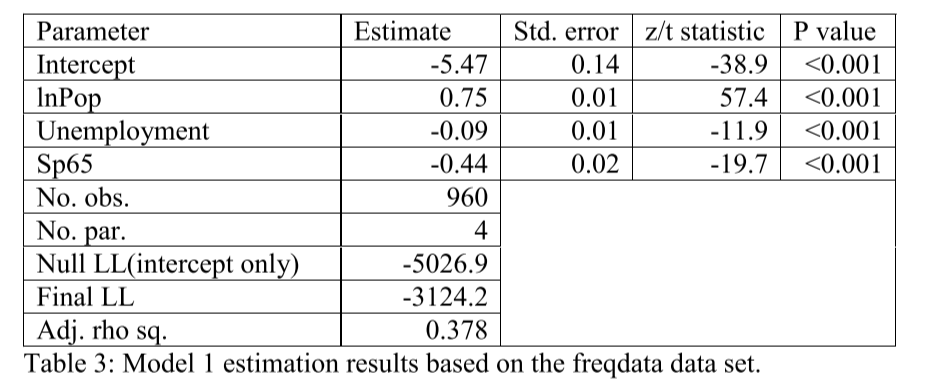
\includegraphics{./images/model_1.png} The first value that we look at,
is the adjusted \(\rho^2\). The formula for \(\rho^2\) is:

\begin{Shaded}
\begin{Highlighting}[]
\DecValTok{1}\SpecialCharTok{{-}}\NormalTok{ (}\SpecialCharTok{{-}}\FloatTok{3124.2}\SpecialCharTok{/{-}}\FloatTok{5026.9}\NormalTok{)}
\end{Highlighting}
\end{Shaded}

\begin{verbatim}
## [1] 0.3785037
\end{verbatim}

\hypertarget{comment-on-interpretation-of-values.}{%
\section{Comment on interpretation of
values.}\label{comment-on-interpretation-of-values.}}

And, similarly to adjusted \(R^2\), it represents the amount of
variation that is explained by the model (Final LL), compared to a model
with no parameters (Null LL). So the explanatory variables included in
the model \emph{log(Population), Unemployment rate, Speed limit of 65
mph law} are explaining some of the variation present in our
measurements of the response-variable, the number of casualties in
traffic among 16 year olds. We also see the p-values reflecting the
t-test for the null-hypothesis of the variables having no influence on
the mean being very low, meaning there is a high degree of statistical
evidence that can let us reject the null-hypothesis of the variables
being insignificant.

We see that population is positively correlated with the response
variable. Which makes sense, as the presence of people is an essential
requirement for people to get into traffic accidents. The unemployment
rate has a negative correlation with the number of accidents. Perhaps
because unemployed people are driving less, or have less access to
vehicles. And finally we see that a speed limit of 65 mph has a reducing
effect on the number of casualties.

\hypertarget{section-c}{%
\section{--------------------- Section C
-----------------------------}\label{section-c}}

\emph{Table 4 shows the estimation results from two other Poisson
regressions with the number of accidents as dependent variable and
additional explanatory variables. Comment on the differences among the
models in Tables 3 and 4 and argue which model you prefer, e.g.~by the
use of LR tests as well as by looking at the signs of parameters.}

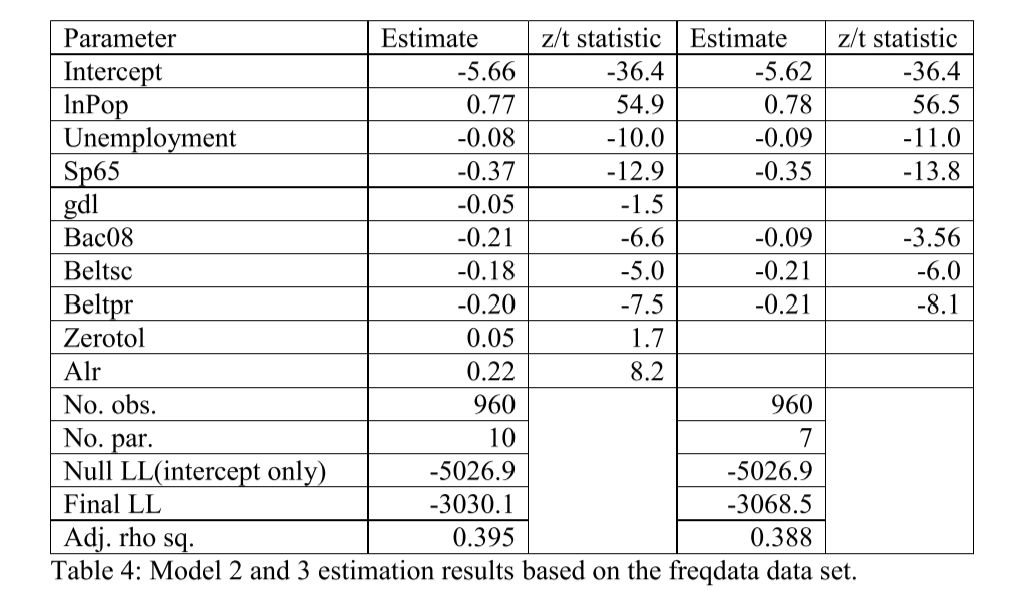
\includegraphics{./images/model_2_and_3.png} Here we see two models. One
model is including all the variables listed in the table, and the other
model has excluded variables \emph{gdl, Zerotol and Alr}. First thing we
notice is that the adjusted \(\rho^2\) is very close for the two models.

We can evaluate the two models against eachother by the log-likelihood
ratio test

\(LLR = -2 * (LL(\hat{\beta}_k) - LL(\hat{\beta}_p))\sim \chi^2_{f=k-p}\)
So the \(LLR\) test statistic is \(\chi^2\) distributed over degrees of
freedom equal to the difference in number of parameters between the two
models

\begin{Shaded}
\begin{Highlighting}[]
\NormalTok{teststat }\OtherTok{\textless{}{-}} \SpecialCharTok{{-}}\DecValTok{2} \SpecialCharTok{*}\NormalTok{ (}\SpecialCharTok{{-}}\FloatTok{3030.1} \SpecialCharTok{{-}}\NormalTok{ (}\SpecialCharTok{{-}}\FloatTok{3068.5}\NormalTok{))}
\NormalTok{teststat}
\end{Highlighting}
\end{Shaded}

\begin{verbatim}
## [1] -76.8
\end{verbatim}

We use the pchisq function to evaluate this statistic over a \(\chi^2\)
distribution with degrees of freedom = \(9-6\)

\begin{Shaded}
\begin{Highlighting}[]
\FunctionTok{pchisq}\NormalTok{(teststat, }\AttributeTok{df =} \DecValTok{9{-}6}\NormalTok{)}
\end{Highlighting}
\end{Shaded}

\begin{verbatim}
## [1] 0
\end{verbatim}

This p-value represents the amount of evidence supporting the
null-hypothesis that the simpler model is equally as good at explaining
the variance in the dataset, as the model with more parameters. With a
p-value of \textasciitilde0, we can reject the null-hypothesis.

So it seems that some of the additional variables \emph{gdl, Zerotol and
Alr} are significant at explaining the amount of variance. The variable
that jumps out as most interesting to explore is alr, as it has the
highest estimated effect. If we look at the correlation matrix we also
see that it is positively correlated with the other two variables
\emph{zerotol} and \emph{gdl}. So we try to reconstruct the extended
model:

\begin{Shaded}
\begin{Highlighting}[]
\NormalTok{poisson\_extended }\OtherTok{\textless{}{-}} \FunctionTok{glm}\NormalTok{(fatal }\SpecialCharTok{\textasciitilde{}}\NormalTok{ lnpop }\SpecialCharTok{+}\NormalTok{ unempl }\SpecialCharTok{+}\NormalTok{ sp65 }\SpecialCharTok{+}\NormalTok{ gdl }\SpecialCharTok{+}\NormalTok{ bac08 }\SpecialCharTok{+}\NormalTok{ beltsc }\SpecialCharTok{+}\NormalTok{ beltpr }\SpecialCharTok{+}\NormalTok{ zerotol }\SpecialCharTok{+}\NormalTok{ alr, }\AttributeTok{data=}\NormalTok{data\_ex2, }\AttributeTok{family=}\FunctionTok{poisson}\NormalTok{(}\AttributeTok{link=}\StringTok{"log"}\NormalTok{))}
\FunctionTok{summary}\NormalTok{(poisson\_extended)}
\end{Highlighting}
\end{Shaded}

\begin{verbatim}
## 
## Call:
## glm(formula = fatal ~ lnpop + unempl + sp65 + gdl + bac08 + beltsc + 
##     beltpr + zerotol + alr, family = poisson(link = "log"), data = data_ex2)
## 
## Deviance Residuals: 
##     Min       1Q   Median       3Q      Max  
## -5.5435  -1.3324  -0.2366   0.8624   5.2923  
## 
## Coefficients:
##             Estimate Std. Error z value Pr(>|z|)    
## (Intercept) -5.65905    0.15539 -36.418  < 2e-16 ***
## lnpop        0.77523    0.01413  54.856  < 2e-16 ***
## unempl      -0.08151    0.00818  -9.965  < 2e-16 ***
## sp65        -0.37294    0.02889 -12.910  < 2e-16 ***
## gdl         -0.04579    0.03078  -1.488    0.137    
## bac08       -0.20948    0.03169  -6.610 3.84e-11 ***
## beltsc      -0.18339    0.03633  -5.048 4.47e-07 ***
## beltpr      -0.20127    0.02690  -7.483 7.28e-14 ***
## zerotol      0.05269    0.03128   1.685    0.092 .  
## alr          0.22297    0.02723   8.188 2.66e-16 ***
## ---
## Signif. codes:  0 '***' 0.001 '**' 0.01 '*' 0.05 '.' 0.1 ' ' 1
## 
## (Dispersion parameter for poisson family taken to be 1)
## 
##     Null deviance: 6670.4  on 959  degrees of freedom
## Residual deviance: 2676.9  on 950  degrees of freedom
## AIC: 6080.3
## 
## Number of Fisher Scoring iterations: 5
\end{verbatim}

And we create the simple model, but this time with \emph{alr} included:

\begin{Shaded}
\begin{Highlighting}[]
\NormalTok{poisson\_simple\_alr }\OtherTok{\textless{}{-}} \FunctionTok{glm}\NormalTok{(fatal }\SpecialCharTok{\textasciitilde{}}\NormalTok{ lnpop }\SpecialCharTok{+}\NormalTok{ unempl }\SpecialCharTok{+}\NormalTok{ sp65 }\SpecialCharTok{+}\NormalTok{ bac08 }\SpecialCharTok{+}\NormalTok{ beltsc }\SpecialCharTok{+}\NormalTok{ beltpr }\SpecialCharTok{+}\NormalTok{ alr, }\AttributeTok{data=}\NormalTok{data\_ex2, }\AttributeTok{family=}\FunctionTok{poisson}\NormalTok{(}\AttributeTok{link=}\StringTok{"log"}\NormalTok{))}
\FunctionTok{summary}\NormalTok{(poisson\_simple\_alr)}
\end{Highlighting}
\end{Shaded}

\begin{verbatim}
## 
## Call:
## glm(formula = fatal ~ lnpop + unempl + sp65 + bac08 + beltsc + 
##     beltpr + alr, family = poisson(link = "log"), data = data_ex2)
## 
## Deviance Residuals: 
##     Min       1Q   Median       3Q      Max  
## -5.4588  -1.3591  -0.2206   0.8570   5.2471  
## 
## Coefficients:
##              Estimate Std. Error z value Pr(>|z|)    
## (Intercept) -5.673754   0.155165 -36.566  < 2e-16 ***
## lnpop        0.779800   0.013902  56.092  < 2e-16 ***
## unempl      -0.084852   0.007844 -10.817  < 2e-16 ***
## sp65        -0.377735   0.025651 -14.726  < 2e-16 ***
## bac08       -0.216825   0.029050  -7.464 8.41e-14 ***
## beltsc      -0.181892   0.035992  -5.054 4.33e-07 ***
## beltpr      -0.202643   0.026448  -7.662 1.83e-14 ***
## alr          0.230353   0.026988   8.535  < 2e-16 ***
## ---
## Signif. codes:  0 '***' 0.001 '**' 0.01 '*' 0.05 '.' 0.1 ' ' 1
## 
## (Dispersion parameter for poisson family taken to be 1)
## 
##     Null deviance: 6670.4  on 959  degrees of freedom
## Residual deviance: 2681.2  on 952  degrees of freedom
## AIC: 6080.6
## 
## Number of Fisher Scoring iterations: 5
\end{verbatim}

And we run the \(LLR\) test for these two models:

\begin{Shaded}
\begin{Highlighting}[]
\FunctionTok{lrtest}\NormalTok{(poisson\_extended, poisson\_simple\_alr)}
\end{Highlighting}
\end{Shaded}

\begin{verbatim}
## Likelihood ratio test
## 
## Model 1: fatal ~ lnpop + unempl + sp65 + gdl + bac08 + beltsc + beltpr + 
##     zerotol + alr
## Model 2: fatal ~ lnpop + unempl + sp65 + bac08 + beltsc + beltpr + alr
##   #Df  LogLik Df  Chisq Pr(>Chisq)
## 1  10 -3030.1                     
## 2   8 -3032.3 -2 4.3267     0.1149
\end{verbatim}

Now we have some evidence supporting the null-hypothesis at a
significance-level of 0.10. We cannot reject the null-hypothesis that
these two models are similar.

\end{document}
